\newpage
\section{Problema 1: Algoritmo Exacto para 2-List Coloring}

\subsection{Descripción de la problemática}
Este ejericicio está centrado en la resolución de un problema particular de coloreo, 2-listColoring. En este caso, cada nodo se puede colorear solo con uno o dos colores específicos. El algoritmo debe determinar si existe o no un coloreo en donde no existen dos nodos consecutivos del mismo color y, en caso afirmativo, encontrar una solución.
Este problema es facilmente reducible a 2-SAT, por lo cual existen algortmos polinomiales que lo resuelven.

\subsection{Resolución propuesta y justificación}
Como mencionamos antes, el problema del 2-ListColoring es facilmente reducible a un problema de 2-SAT, y en esto se basa el algoritmo implementado. Si existe una coloración posible, entonces el hecho de que un determinado nodo esté pintado de un color implica que ninguno de sus vecinos esta pintado del mismo. Además, si un color tenía dos opciones posibles, el nodo esta pintado de un color A si y solo si no esta pintado del color B.
El 2-SAT se representa con un grafo dirigido en donde un nodo A (que representa una premisa) apunta a un nodo B si y solo si A implica B.

Una vez construido el grafo dirigido que representa el problema, lo primero que hace el algoritmo es encontrar componentes fuertemente conexas en el grafo. En este contexto, una componente fuertemente conexa representa un conjunto de propociones de las cuales se puede afirmar que todas son válidas o todas son falsas. Consecuentemente, se construye un grafo dirigido en donde cada nodo representa una componente fuertemente dirigida del grafo anterior; logicamente, este segundo grafo no contiene ninguna componente fuertemente conexa. 
El algoritmo debe chequear, además, si se incluye en una misma componente conexa una propoción (asignación de un color a un nodo) y su negación, en cuyo caso el nodo que representa dicha componente debe tener un valor de verdad negativo. Además, el algoritmo registra, para cada componente, cual es la componente que representa su negación, es decir, que contiene la negación de las variables de la primera.
Finalmente comienzan a fijarse los valores de verdad. Cuando se fija un valor para un nodo determinado, el nodo que contiene los valores contrarios se fija en el valor opuesto. Además, si un nodo se fija en false, todos los nodos que implican al mismo deben fijarse en false (igual recursivamente) y si se fija en true, todos los que son implicados por el mismo deven fijarse en true. Si el algoritmo encuentra una contradicción (es decir, un nodo que debía setearse en false fue seteado en true o viceversa), determina que el problema no teiene una solución válida.


\subsection{Análisis de la complejidad}
El grafo dirigido contiene a los sumo cuatro veces más nodos que el grafo de entrada, y el grafo compacto tiene a los sumo tantos nodos como el grafo dirigido. Por lo tanto, podemos afirmar que, sea n la cantidad de nodos inicial, n' la cantidad de nodos del grafo dirigido y n'' la cantidad de nodos del grafo compacto, $\mathcal{O}(f(n)) = \mathcal{O}(f(n')) = \mathcal{O}(f(n''))$ (si no se conocen datos adicionales para la entrada).

Generar el grafo dirigido a partir del grafo de entrada tiene una complejidad de $\mathcal{O}(n^2\log{n})$, ya que para cada nodo del grafo, es necesario crear los nodos dirigidos que lo representan y definir sus aristas con otros nodos. A medida que se van creando, los nodos se guardan y se buscan en un TreeSet.

El algoritmo utilizado para encontrar las componentes fuertemente conexas no recorre más de dos veces todos los nodos, por lo cual su complejidad es lineal, al igual que el algoritmo que determina el valor de verdad de los nodos compactos.

\subsection{Código fuente}

A continuación se incluyen las partes más relevantes del código.\\
La clase lector se encarga de leer la entrada y transforla en un grafo. Como en los test de complejidad es importante no medir el tiempo que se tarda en cargar el archivo en memoria, el Lector posee funciones para cargar la información sin procesar.
\lstinputlisting[name=pp, numbers=left, frame=lines, firstline=105, lastline=161]{../ej1/src/Lector.java}
Los metodos que construyen el coloreo se encuentran en Calculador_de_Coloracion_Ej1 \\
\lstinputlisting[name=gr, numbers=left, frame=lines, firstline=114, lastline=220]{../ej1/src/Calculador\string_de\string_Coloracion\string_Ej1.java}

\subsection{Experimentación}
Casos de test:
\subsubsection{El triángulo}
En este test existen tres nodos interconextados en donde cada nodo comparte un color con uno de sus vecinos. El algoritmo debería encontrar la única solución posible.
Posteriormente, se le añade al triangulo un nodo extra vecino del primero con el color con el cual estaba pintado el primero, con lo cual no existe solución.
\subsubsection{El pentagono}
En esta oportunidad, se dibuja un k5. Cada nodo tiene como opción un color que no se repite en sus compañeros y otro que es compartido por más de uno. El algoritmo debería encontrar una solución
\subsubsection{El señor de los anillos}
En este caso se prueba un ciclo de seis nodos. A los pares se les asigna 0 y a los impares uno, y además todos poseen un segundo color que comparten con uno de sus vecinos. Como el grafo es bipartito, el algoritmo debería hallar una solución.
\subsubsection{Grafos bipartitos completos}
Otro de los casos se basa en generar grafos bipartitos completos. En este caso, se les asigna a todos los nodos 0 y 1. Como un grafo bipartito (en particular, uno completo) puede colorearse con dos colores, el algoritmo deberia encontrar una solución para el mismo. Posteriormente, se le añade al grafico una arista que une dos nodos que no estaban conectados, con lo que el grafo deja de ser bipartito y se necesitan 3 colores para colorearlo. En este caso, el algoritmo debería determinar que no existe solución.

\subsubsection{Testeos de complejidad}
Para testear la complejidad, se generan grafos al azar en donde todos los nodos poseen como opciones de coloreo a un color que no se repite en los demás nodos y otro que es seleccionado al azar. En una de las estrrategias se deja fija la cantidad de aristas, en otra se fija la cantidad de nodos, y en la otro se incrementan las aristas y los nodos en igual proporción.

\subsubsection{Complejidad en grafos completos}
En un último caso se generan grafos completos en donde se a incrementando la cantidad de nodos (y, logicamente, de aristas). Debido al consumo de memoria, este último caso se ha testeado con valores inferiores que al resto de los test.

\subsubsection{Constrastación Empírica de la complejidad}


% \begin{figure}[H]
% 	\centering
%  	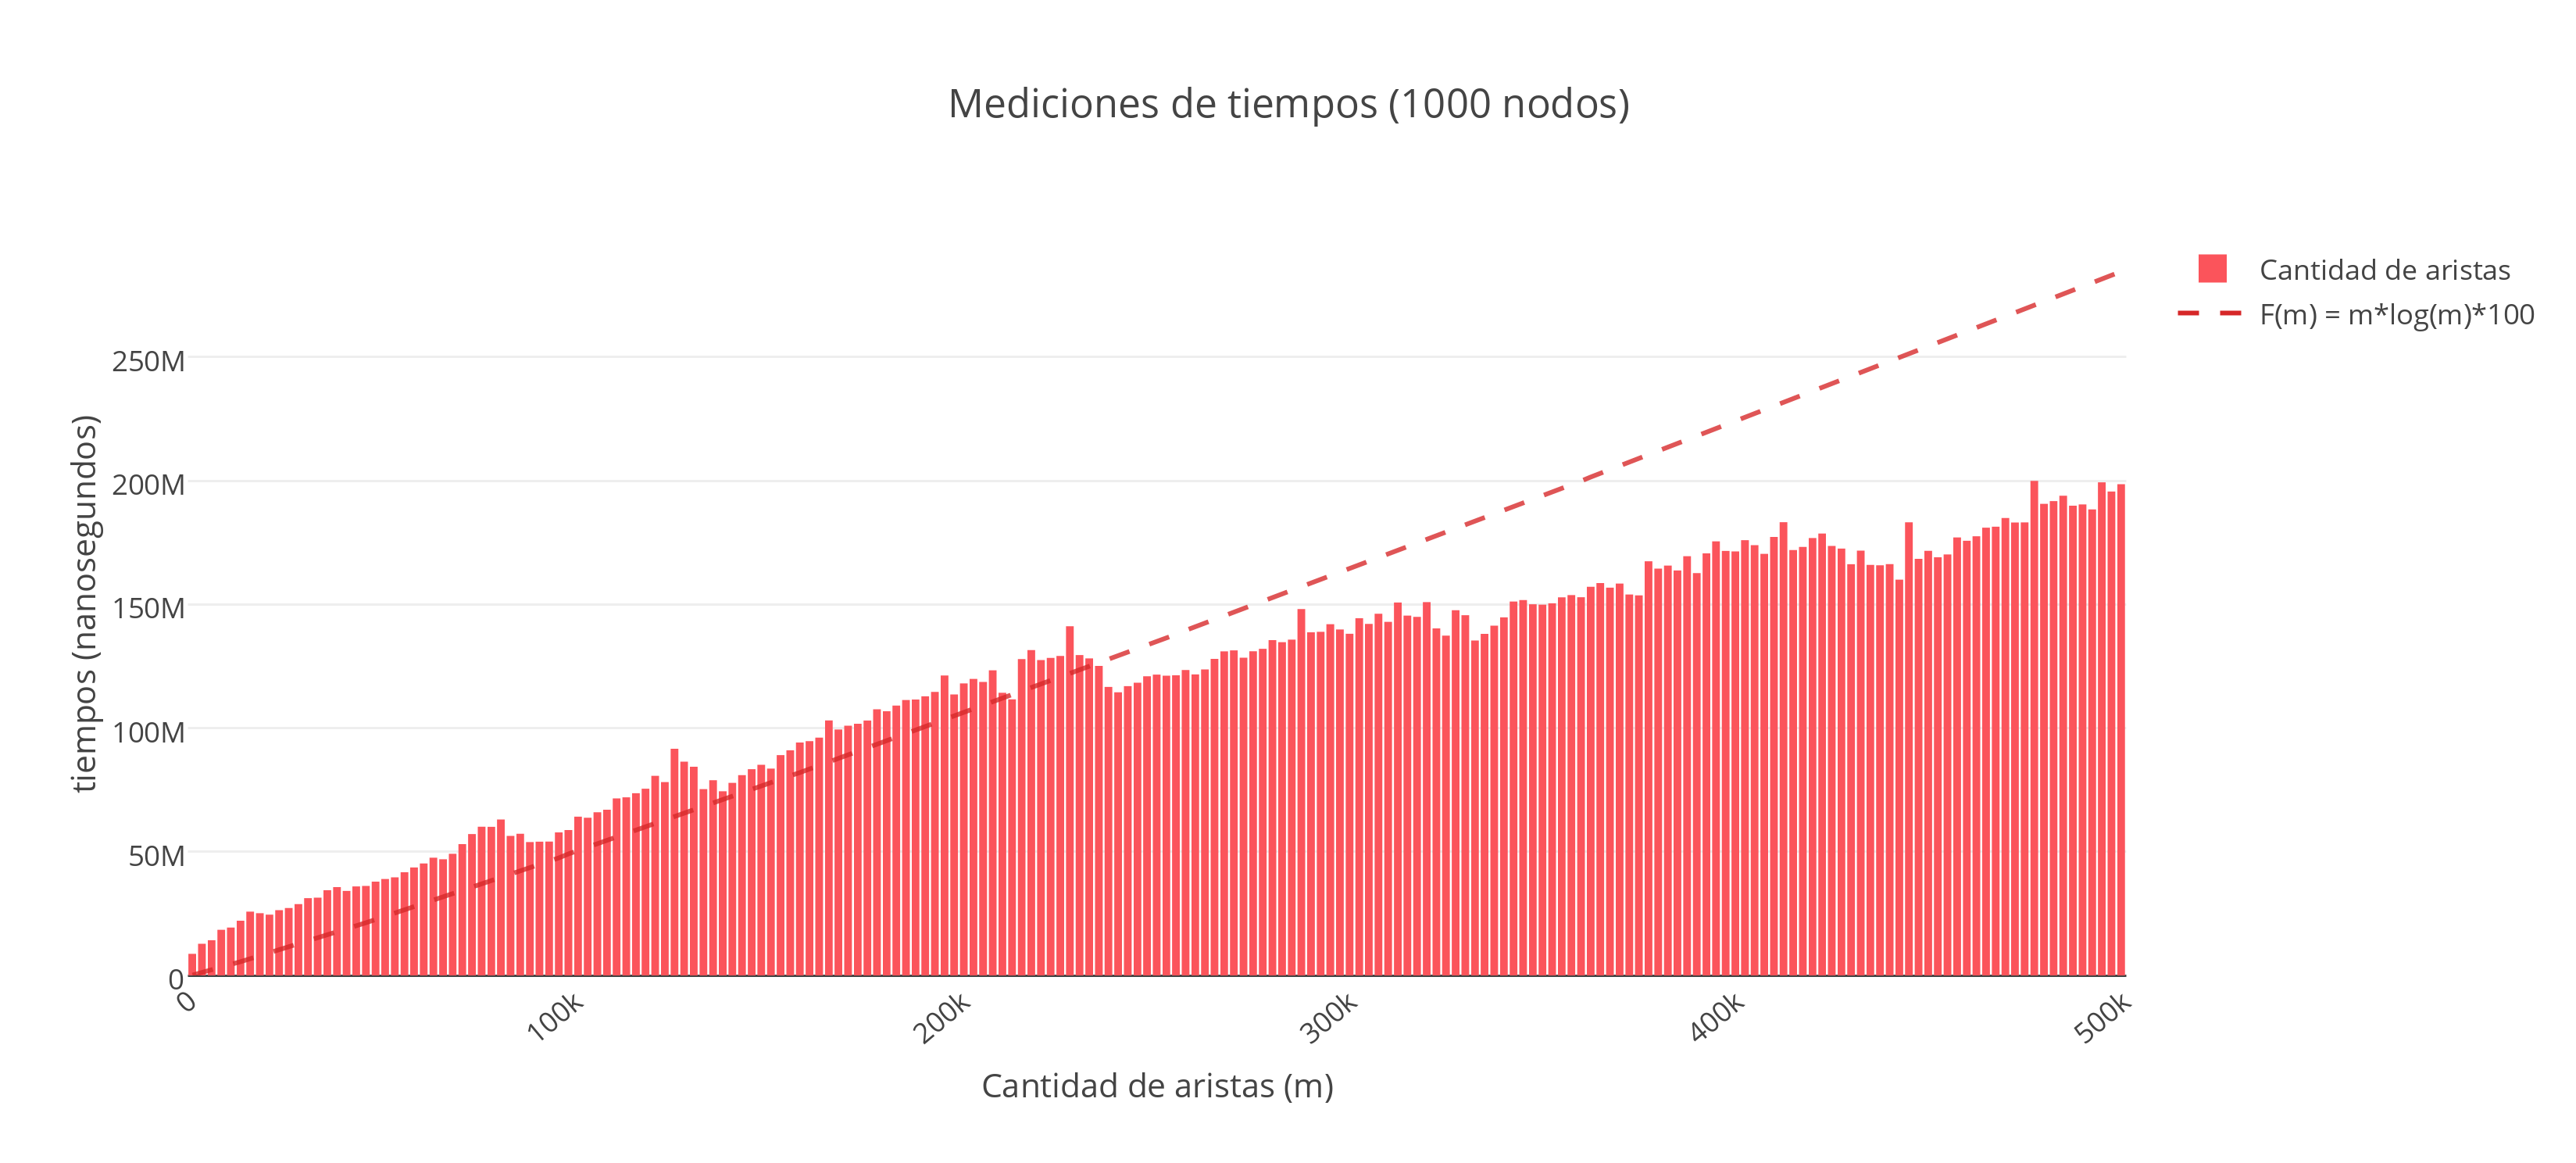
\includegraphics[scale=0.6]{imagenes/ej3/tiempos1000B.png}
% 	\caption{Medición de tiempo promedio con $n$ fijo en 1000}
% 	%\label{tiemposprom}
%  \end{figure}